This section will discuss the discretisation of the plant model and the controllers designed in \cref{sec:continuous}. First, \cref{sec:plantdiscretisation} treats the discretisation of the plant model separately. Then, \cref{sec:discretisecontrollers} follows with the discretisation of the controllers.\footnote{A word of caution must be emphasised about this section: the numerical results for the discretised models and controllers naturally only carry a finite precision. Since discrete-time models are notorious for being sensitive to truncation errors; it is \textbf{not} advised to use these numerical results directly for reproduction.}

\subsection{Discretisation of the plant\textnormal{\phantom{xxx}(Question 3)}}
\label{sec:plantdiscretisation}
The transfer function of the plant (\cref{eq:plant}), has the state-space realization in the following canonical form:
\begin{equation}
    \begin{aligned}
        \dv{x}{t} &= \mqty(0 & 1 & 0 \\ 0 & 0 & 1 \\ 0 & -144 & -24)x + \mqty(0 \\ 1 \\ -4)u\\
        y &= \mqty(1 & 0 & 0)x
    \end{aligned}
\end{equation}
It is known that the output of the system represents the orientation of the space station. From the state space description, it is therefore clear that the first state must also be equal to this orientation. Then, from the first state-space equation it is clear that $\dv{x_1}{t} = x_2$; which means that $x_2$ represents the angular velocity associated with the orientation of the spacecraft. Again, $\dv{x_2}{t} = x_3 + u$. Clearly, $u$ acts as a torque on the change in angular velocity; $x_3$ must therefore represent the angular acceleration. The third equation states that $\dv{x_3}{t} = -144x_2 - 24x_3 -4u$. It is not entirely evident what this equation represents, but it introduces some coupling between the angular velocity and the angular acceleration of the system. Therefore, one might guess that this equation represent some gyroscopic effect that is present in the rotational dynamics of the system --- a common way to adjust the attitude of spacecraft is by means of so-called Control Moment Gyroscopes.

\paragraph{Discretization of the plant}
To find a discrete-time state-space representation of the plant a suitable sampling period $h$ has to be chosen. The sampling time was based on the location of the fastest poles $s = -12$ and their corresponding time constant $\tau$ such that $h = \sfrac{\tau}{5}$. Based on this rule, a sampling period of $h = \SI{0.017}{\second}$ was chosen. Using the \textsc{Matlab}-command \texttt{c2d} with the zero-order hold method, the resulting discrete-time state-space model is:
\begin{equation}
    \begin{gathered}
        x(k+1) = \Phi x(k) + \Gamma u(k) \qquad y(k) = Cx(k) + Du(k)\\
        \Phi = 
        \begin{pmatrix}   
            0.818730757429643 &  0.341137813782492 &   0\\
            0 & 0.818730748726321 & 0\\
            0  &  0 &  1\\
        \end{pmatrix}\quad
        \Gamma = \begin{pmatrix}
            -0.097796027122327\\
            -0.032225642649731\\
             0.111910703183245\\
        \end{pmatrix}\\
        C = \mqty(0.012500000378703 & 0.029687499840546 & 0.020684481010047) \quad D = 0
    \end{gathered}
\end{equation}
\Cref{fig:q3_dt_plant_impulse} shows a comparison between the impulse response of the continuous system and the discrete system.
\begin{figure}
    \centering
    \includegraphics[]{media/q3/dt_plant_impulse.eps}
    \caption{Comparison between the impulse response of the continuous-time plant and the sampled discrete-time plant ($h = \SI{0.017}{\second}$).}
    \label{fig:q3_dt_plant_impulse}
\end{figure}

\subsection{Discretisation of the controllers \textnormal{\phantom{xxx}(Question 4)}}
\label{sec:discretisecontrollers}
Now, both the controllers from \cref{sec:continuoustracking,sec:continuousdisturbance} and the plant are discretised separately, after which a closed loop response simulation is performed. Again, another rule of thumb is used from \textcite[317]{astrom} for PID-type controllers:
\begin{equation}
    \frac{hN}{T_d} \approx 0.2 \text{ to } 0.6
    \label{eq:samplingpidrule}
\end{equation}
In this case, $N = 10$ was taken in accordance with \textcite{astrom}. Of course, the controller designs were of type PIDD so some care had to be taken when using this method.

\paragraph{Tracking controller}
The tracking controller was discretised using the Tustin approximation while the plant was discretised using the zero-order hold method (both with identical sampling period). The sampling period was computed using \cref{eq:samplingpidrule} with the smallest of the two $T_d$'s. The resulting sampling time was increased slightly more to obtain also a reasonable number of samples per rise time. The sampling time used was $h = \SI{0.0014}{\second}$. The resulting simulation is shown in \cref{fig:q4_dt_tracking}; the discretised controller shows comparable performance with slightly higher overshoot and settling time.
\begin{figure}[ht]
    \centering
    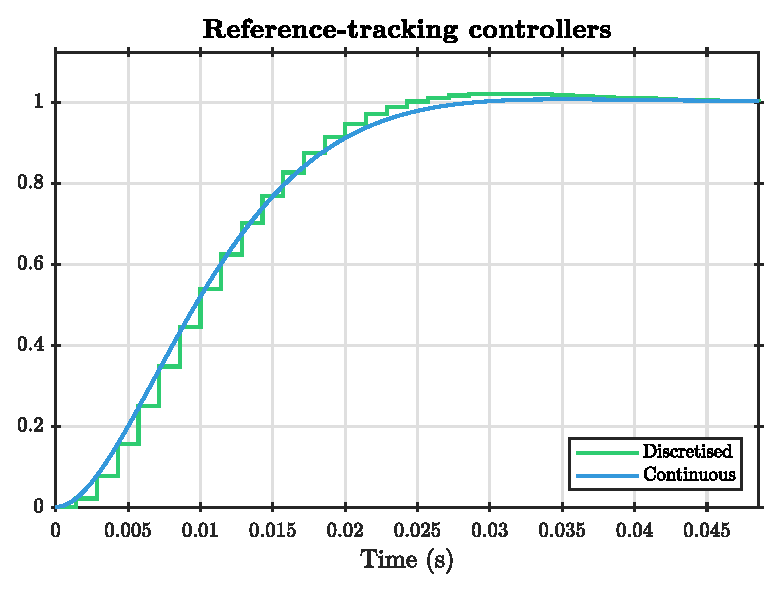
\includegraphics[]{media/q4/dt_tracking.eps}
    \caption{$h = \SI{0.0014}{\second}$}
    \label{fig:q4_dt_tracking}
\end{figure}

\begin{figure}[ht]
    \centering
    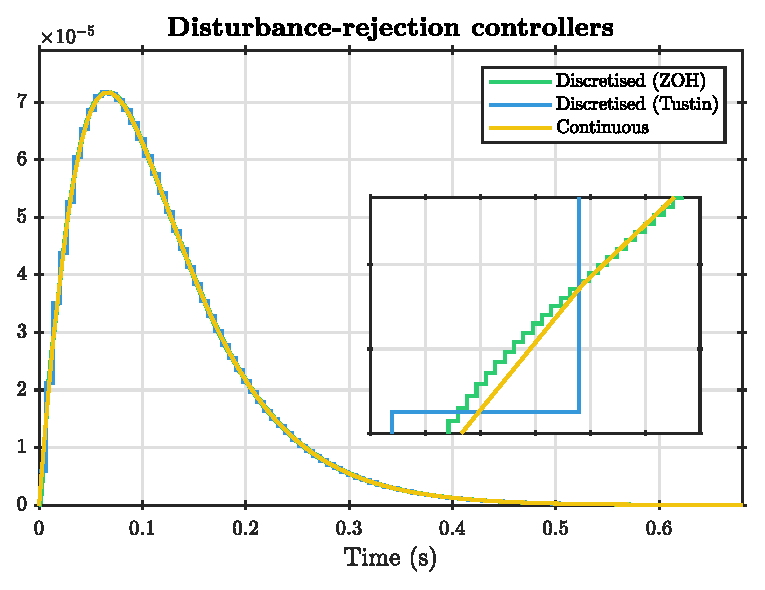
\includegraphics[]{media/q4/dt_distrej.eps}
    \caption{$h = \SI{0.0012}{\second}$}
    \label{fig:q4_dt_distrej}
\end{figure}
\paragraph{Disturbance rejection controller}
Like the tracking controller, sampling period was based on the smallest of the two $T_d$'s of the PIDD controller. This resulted in a sampling time of $h = \SI{0.0012}{\second}$. However, the time constant of a step response is several orders of magnitude larger; so a larger sampling period may also be suitable to capture the same response. The meager stability margins of this controller did not allow to discretise the plant with zero-order hold for this larger sampling period due to excessive warping of the phase curve. Hence, the Tustin approximation was used for both the plant and the controller with a sampling time 10 times larger then the one used for the zero-order hold method. 

\Cref{fig:q4_dt_distrej} shows a comparison between the three methods: the continuous plant and controller, the plant discretised with ZOH and the controller with Tustin using the small $h$, and both discretised with Tustin using a larger sampling period. From the global perspective the first two responses are virtually indistinguishable (note the close-up view), so the Tustin approxmation definitely allows to capture the shape of the response with reasonable sampling time. 

Because the plant surpresses higher frequencies, one can gather from \cref{eq:disttf} that the response of the ouput will indeed be slow. The underlying dynamics of the loop and the controller are much faster, so in this case one should not rely on the time response to determine the sampling time. This is why the choice was made to use the \textit{first sampling frequency and the ZOH method} after all to make sure that the fastest dynamics of the PIDD controller are represented in the discrete system to a sufficient degree. 